\documentclass[10pt,a4paper]{article}
\usepackage[utf8]{inputenc}
\usepackage[english]{babel}
\usepackage{textcomp}
\usepackage{titling}
\newcommand{\subtitle}[1]{%
  \posttitle{%
    \par\end{center}
    \begin{center}\large#1\end{center}
    \vskip0.5em}%
}
\usepackage{amsmath}
\usepackage{amsfonts}
\usepackage{amssymb}
\usepackage{graphicx}
\usepackage{lmodern} 
% set colors for links and URLs
\usepackage[
	colorlinks=true,
	urlcolor=blue,
	linkcolor=green
]{hyperref}
\author{-- prozumr --}
\title{Meaningful Version Numbering}
\subtitle{Versioning Rules for \linebreak RLOTTO}

\begin{document}
\maketitle
\pagebreak[4]
\section*{Abstract}
Objective of this document is to describe conventions used as basic concept for handling of version numbers in a particular open source software project called RLOTTO as published on github\footnote{\url{https://github.com/prozumr/RLOTTO2}}. Moreover the concept described herein has the potential to be generalized and used for other software projects even though this is not the primary intention of this document. 
\\
Please note: The concept or approach described in this document is up to a significant extent derived from another well known concept called \textit{Semantic Versioning}\footnote{\url{https://semver.org/}}. 

\section*{Introduction}

The need for version numbers in the world of software development is obvious and does not need any further explanation. However a strict set of rules and regulations how to approach versioning and how to determine version numbers is neither trivial nor self-evident and requires a bunch of considerations and decisions. 
\\
The underlying fundamental pillars of the resulting outcome as described in this document were a) the concept of Semantic Versioning by Tom Preston-Werner and b) my own set of requirements as described in section \textit{Basic Requirements}.

One may ask: why not adopting Semantic versioning completely "as-is"? The honest answer is that I was struggeling with the term of "incompatible API changes" assuming that this does not make much sense in case of such a small console Program as RLOTTO that does not interact with any other kind of other systems or protocols. Some changes to the definition for the major version number were required to fit to specific needs as described in section \textit{Meaningful Version Numbering}.

\section*{Basic Requirements}

The following set of basic requirements have been formulated for issue \# 11 on github:

\begin{enumerate}
\item A unique version number
\item A concept (with strictly formalized rules) using components in the version number that reflect major/minor releases and eventually a build or patch number
\item Mapping of version number to github commit/release must be possible
\item Easy maintenance of the version number
\end{enumerate}

Most comprehensive in this enumeration is the second item. Luckily \textit{Semantic Versioning} is fully covering this requirement. However and as already mentioned some adjustments were needed to fulfill the specific demand of software projects with no defined or documented API. This is described in the section after the next.

\section*{Unique Version Number}

Naturally a unique version number is needed but what does it exactly mean? Here are some specifics:

\begin{itemize}
\item Any of two different software versions must not have the same version number.
\item The version number always applies to all files of the source code. I.e. in a set of source code files all individual files have the same version number.
\item The version number is not random but following defined rules for generating the new version number by an increment of the previous version number.
\item Usage of a natural number just by incrementing by one (or any other constant increment) for a new version could be misleading even though fulfilling the requirement of uniqueness: tiny minor changes and huge fundamental changes would not be capable of being differntiated just by the version number.
\end{itemize}

\section*{Meaningful Version Numbering}

Semantic versioning is based on two elements: Meaningful version numbers and a set of rules and that dictate how to increment these version numbers. Embedding more meaning in more numbers is an obvious concept and used by Semantic Versioning as follows:


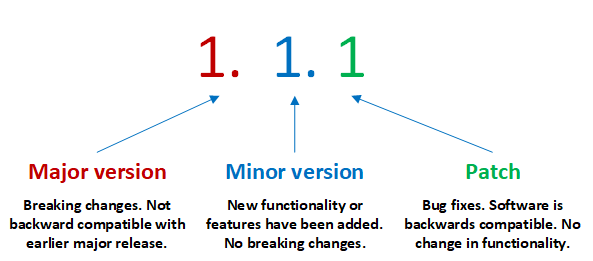
\includegraphics[scale=0.75]{SemanticVersioning.png} 
\\

Thus three components are used to build the complete version string:
\begin{enumerate}
\item MAJOR version for breaking changes not backward compatible to earlier releases
\item MINOR version for adding functionality in a backwards-compatible manner, and
\item PATCH version for backwards-compatible bug fixes.
\end{enumerate}

Additional labels for pre-release are available as extensions to the \linebreak MAJOR.MINOR.PATCH format:

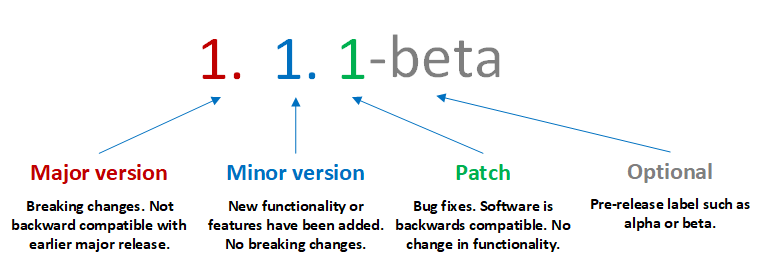
\includegraphics[scale=0.65]{SemanticVersioning2.png} 
\\
A more precise definition which of the version number components should be changed and how to increment the number is given in the following section.

\section*{Meaningful Version Numbering Specification}

As already discussed in the introduction of this document this versioning approach can be called a light-weight, slightly adjusted version of the original Semantic Versioning concept by Tom Preston-Werner. The main difference is that rule No 1 of Semantic Dersioning is neglected ("Software using Semantic Versioning MUST declare a public API."). Instead the conditions when a change of the major version is required is described in a different manner. Please see below for a complete set of rules required for "Meaningful Version Numbering".
\\

The key words “MUST”, “MUST NOT”, “REQUIRED”, “SHALL”, “SHALL NOT”, “SHOULD”, “SHOULD NOT”, “RECOMMENDED”, “MAY”, and “OPTIONAL” in this document are to be interpreted as described in RFC 2119\footnote{\url{https://tools.ietf.org/html/rfc2119}}.

\begin{enumerate}

\item Software using Meaningful Versioning Numbering \textbf{MUST NOT} declare a public API. This is reflecting the author's belief that it is not possible to rely fully on a deterministic an mechanic approach to cover all scenarios by a set of rules to guarantee the best way of consistent versioning. See also article \href{https://gist.github.com/jashkenas/cbd2b088e20279ae2c8e}{Why Semantic Versioning Isn't} for details on this point of view. Instead pretty precise rules and guideline are given below.

\item  A normal version number MUST take the form X.Y.Z where X, Y, and Z are non-negative integers, and MUST NOT contain leading zeroes. X is the major version, Y is the minor version, and Z is the patch version. Each element MUST increase numerically. For instance: $1.9.0 \Rightarrow 1.10.0 \Rightarrow 1.11.0$.

\item Once a versioned package has been released, the contents of that version MUST NOT be modified. Any modifications MUST be released as a new version.

\item Major version zero (0.y.z) is for initial development. Anything may change at any time. The code base should not be considered stable.

\item Version 1.0.0 defines the public released version - sometimes also called 'Production Release'. The way in which the version number is incremented after this release is dependent on this version as baseline.

\item Patch version Z $(x.y.Z | x > 0)$ 
\begin{itemize}
\item MUST be incremented if only backwards compatible bug fixes are introduced.
\item A bug fix is defined as an internal change that fixes incorrect behavior.
\end{itemize}

\item Minor version Y $(x.Y.z | x > 0)$  
\begin{itemize}
\item MUST be incremented if new, backwards compatible functionality is introduced that is considered as NOT 'big' enough to justify a change of the major version. Intentionally this leaves room for human interpretation.
\item It MUST be incremented if any public functionality is marked as deprecated.
\item It MAY include patch level changes.
\item Patch version MUST be reset to 0 when minor version is incremented.
\end{itemize}

\item Major version X $(X.y.z | X > 0)$  
\begin{itemize}
\item MUST be incremented if any backwards incompatible functional or non-functional changes are introduced.
\item MUST be incremented if any backwards compatible functional or non functional changes are introduced that are considered to be too 'big' to justify just a minor version change. Intentionally this leaves room for human interpretation.
\item It MAY include minor and patch level changes.
\item Patch and minor version MUST be reset to 0 when major version is incremented.
\end{itemize}

A good indicator for a backwards incompatible change is a non-consistent behavior or even a malfunction after a software update. E.g. The updated version cannot read the input data stored in the database or on the file system anymore.

\item A pre-release version MUST be denoted by appending suffix like 'alpha' or 'beta'. A pre-release version indicates that the version is unstable and might not satisfy the intended compatibility requirements as denoted by its associated normal version. The absence of the pre-release suffix indicates a normal version - sometimes also called 'Production Release'. Examples: 1.0.1-alpha, 1.1.2-beta.


\end{enumerate}

\section*{Mapping of version number to github commit/release}

Git respectively github assigns a unique identifier - called  commit id or commit hash value -  to any set of source code files by the git commit process. This raises immediately at least two questions:
\begin{enumerate}
\item Can we use the commit id as release number?
\item How to map a certain commit/version to a release number?
\end{enumerate}

Apparently the second question is only relevant in case the first one has to be negated. So why not use the commit id as release or version number?

Well, these git commit IDs are not very helpful for the human eye and mind and can be quite confusing. Humans can neither memorize such a forty-character number nor recognize any sequence of version nor getting any other meaning just by the number.

Also there is another even more principal reason why the git commit ID is not a good choice to be a release number: in case the release number should appear in the software itself - i.e. the release number should be visible for users - it needs to be include or 'hardcoded' in the source code before compiling the code. However this is not possible since the commit ID is not provided before the actual commit. In other words you would have to change the source code after the commit which makes the commit ID invalid.

So what is the conclusion? How to map commit ID and release number and how does the entire release number process look like?
\\
\\
This is the proposed release number process as it is used for RLOTTO:
\\
 
\fbox{
\parbox{0.9\linewidth}{
\begin{enumerate}
\item Determine the new release number(s) in semantic format MAJOR.MINOR.PATCH-PRE-RELEASE by rules as defined in section \textit{Meaningful Version Numbering Specification}
\item Hardcode your release number inside the source code as described in section \textit{Source Code Implementation}
\item Commit this version of your source code to github
\item Tag the commit on github\footnotemark as new release by using exactly the same release string as hardcoded in the source code
\end{enumerate}}
}
\\
\\ 
\\ 
The following and last section addresses the concrete implementation of the release number in the source code.

\section*{Source Code Implementation}


RLOTTO uses a dedicated header file to maintain version numbers within the source code. The file is called \texttt{version.h}. Within \texttt{version.h} dedicated variables are defined:
\begin{itemize}
\item \texttt{MAJOR} to maintain the major component of the version number.
\item \texttt{MINOR} to maintain the minor component of the version number.
\item \texttt{PATCH} to maintain the patch component of the version number.
\item \texttt{STAGE} to maintain the (pre-) release status component of the version number.
\end{itemize}

The range of values for \texttt{STAGE} just includes "alpha", "beta" and "production". These four variables are used to build the version number string that appears on the user interface (console window or shell) during start of RLOTTO. In case \texttt{STAGE} is not set (empty) or has any other value than "alpha", "beta" or "production" the program throws a warning message during start: "Release state undefined". In case \texttt{STAGE} is set to "production" the release state is not indicated on the user interface bust just shows the version number MAJOR.MINOR.PATCH. In case STAGE is set to a pre-release it is shown on the user interface like MAJOR.MINOR.PATCH-alpha or MAJOR.MINOR.PATCH-beta.
\\

The full version number is generated by a \texttt{printf} statement inside the function \texttt{welcome()} in \texttt{rlotto.c} considering the three different scenarios as described above (wrong or missing value for \texttt{STAGE}, pre-release, production release).
\\

The full version number is used once again by a \texttt{fprintf} statement inside the function \texttt{evaluateTicket(void)} in \texttt{evaluate.c} for generating the header of the result file.
\\

In any case the maintenance of the version number and release state is easy and requires just to update  the variables \texttt{MAJOR}, \texttt{MINOR}, \texttt{PATCH} and \texttt{STAGE} in \texttt{version.h}. 


% FOOTNOTES ----------------------------------
\footnotetext[4]{See also \href{https://git-scm.com/book/en/v2/Git-Basics-Tagging}{Git Basics - Tagging}}

\end{document}
